% CHIL 2026 Submission
% Conference on Health, Inference, and Learning
% Using PMLR/JMLR style (CHIL uses this format)

\documentclass[twoside]{article}

% ============================================================================
% PACKAGES
% ============================================================================
\usepackage[utf8]{inputenc}
\usepackage{amsmath,amssymb,amsfonts}
\usepackage{graphicx}
\usepackage{booktabs}
\usepackage{hyperref}
\usepackage{algorithm}
\usepackage{algorithmic}
\usepackage{float}
\usepackage{subfigure}
\usepackage{multirow}
\usepackage{xcolor}

% Page layout (approximate CHIL/PMLR style)
\usepackage[margin=1in]{geometry}

% Hyperlinks
\hypersetup{
    colorlinks=true,
    linkcolor=blue!70!black,
    citecolor=blue!70!black,
    urlcolor=blue!70!black
}

% ============================================================================
% ANONYMIZATION - Remove for camera-ready
% ============================================================================
% For submission, paper must be anonymous
\newcommand{\theauthors}{Anonymous}
\newcommand{\theaffiliation}{Anonymous Institution}

% ============================================================================
% DOCUMENT
% ============================================================================
\title{Hierarchical Path Reasoning in Biomedical Knowledge Graphs:\\
Multi-Hop Prediction of Disease-Phenotype Associations}

\author{\theauthors}

\date{}

\begin{document}

\maketitle

% ============================================================================
\begin{abstract}
Predicting associations between diseases and phenotypes requires reasoning over complex multi-hop biological pathways. We present \textbf{PathHeteroGNN}, a heterogeneous graph neural network designed for multi-scale biological reasoning in knowledge graphs. Evaluating on PrimeKG (129K nodes, 8M edges), we extract disease-specific subgraphs and predict gene-phenotype associations through intermediate biological entities (metabolites, pathways). On a celiac disease case study, our model achieves AUROC of $0.XXX \pm 0.XXX$, outperforming TransE, DistMult, and R-GCN baselines by $X$--$X$\%. Systematic ablation studies reveal that metabolite-mediated pathways contribute $X$\% to prediction accuracy, while microbiome connections contribute $X$\%. We validate top predictions against held-out literature evidence, achieving $X$\% precision on known associations. Our results demonstrate that explicit modeling of biological hierarchies improves both predictive performance and interpretability for disease mechanism discovery.
\end{abstract}

% ============================================================================
\section{Introduction}

Understanding the biological mechanisms underlying disease requires reasoning across multiple scales—from molecular interactions to cellular processes to systemic manifestations. This is particularly challenging for complex diseases with multi-organ involvement, such as celiac disease, where intestinal inflammation produces neurological symptoms in 10–22\% of patients through incompletely understood mechanisms \citep{lebwohl2018celiac}.

Biomedical knowledge graphs (KGs) provide a natural framework for integrating heterogeneous biological relationships. Recent large-scale KGs such as PrimeKG \citep{chandak2023primekg} contain millions of edges connecting diseases, genes, drugs, phenotypes, and biological processes. However, standard link prediction approaches treat all edges uniformly, failing to capture the hierarchical nature of biological systems.

We identify three key challenges for disease-phenotype prediction in biomedical KGs:

\begin{enumerate}
    \item \textbf{Multi-hop reasoning}: Disease-phenotype associations often operate through intermediate entities (genes, metabolites, pathways) requiring multi-hop inference.
    
    \item \textbf{Biological hierarchy}: Different relationship types operate at different scales (molecular, cellular, organ-level), suggesting that different message-passing depths may be appropriate.
    
    \item \textbf{Interpretability}: Clinical utility requires not just predictions but explanations—which pathways connect a disease to a phenotype?
\end{enumerate}

We present \textbf{PathHeteroGNN}, a heterogeneous GNN architecture that explicitly models multi-hop biological pathways for disease-phenotype prediction. Our contributions are:

\begin{itemize}
    \item A \textbf{hierarchical message-passing} architecture that learns different aggregation depths for different biological relationship types.
    
    \item Comprehensive evaluation on \textbf{PrimeKG} (129K nodes, 8M edges), comparing against 5+ baselines with statistical significance tests.
    
    \item \textbf{Ablation studies} quantifying the contribution of different biological intermediates (metabolites, pathways, gene families).
    
    \item \textbf{Biological validation} through literature-based held-out evaluation and pathway enrichment analysis.
    
    \item A detailed \textbf{case study on celiac disease}, demonstrating how the model identifies gut-brain axis mechanisms.
\end{itemize}

% ============================================================================
\section{Related Work}

\subsection{Knowledge Graph Embedding}

Translational models (TransE, TransR, RotatE) learn entity embeddings where relationships are modeled as geometric operations \citep{bordes2013transe}. Semantic matching models (DistMult, ComplEx) use bilinear scoring functions \citep{yang2015distmult}. While effective on benchmark KGs, these methods do not explicitly model multi-hop reasoning.

\subsection{Graph Neural Networks for Biomedical KGs}

R-GCN \citep{schlichtkrull2018rgcn} extends GCNs to heterogeneous graphs with relation-specific transformations. CompGCN \citep{vashishth2020compgcn} jointly embeds nodes and relations. HGT \citep{hu2020hgt} uses heterogeneous attention mechanisms. These methods have been applied to drug-target prediction \citep{zhang2022graph} but typically treat all edges uniformly.

\subsection{Disease Mechanism Discovery}

Recent work has applied GNNs to disease-gene association \citep{} and drug repurposing \citep{}. However, few studies explicitly model the hierarchical biological structure or validate predictions against independent evidence.

% ============================================================================
\section{Methods}

\subsection{Problem Formulation}

Let $\mathcal{G} = (\mathcal{V}, \mathcal{E}, \mathcal{T}_V, \mathcal{T}_E)$ be a heterogeneous knowledge graph where $\mathcal{V}$ is the set of nodes, $\mathcal{E}$ the set of edges, $\mathcal{T}_V$ node types, and $\mathcal{T}_E$ edge types. Given observed edges $\mathcal{E}_{train}$, we predict unobserved edges in $\mathcal{E}_{test}$, specifically focusing on gene-phenotype associations.

\subsection{Data: PrimeKG}

We use PrimeKG \citep{chandak2023primekg}, a comprehensive biomedical KG containing:
\begin{itemize}
    \item 129,375 nodes across 10 types (diseases, genes, drugs, phenotypes, pathways, etc.)
    \item 8,100,498 edges across 30 relationship types
\end{itemize}

For efficient experimentation, we extract disease-specific subgraphs using $k$-hop neighborhood expansion from seed disease nodes. For our celiac disease case study, we extract nodes within 3 hops of celiac disease (MONDO:0005130), yielding a subgraph of approximately [X] nodes and [X] edges.

\begin{figure}[t]
    \centering
    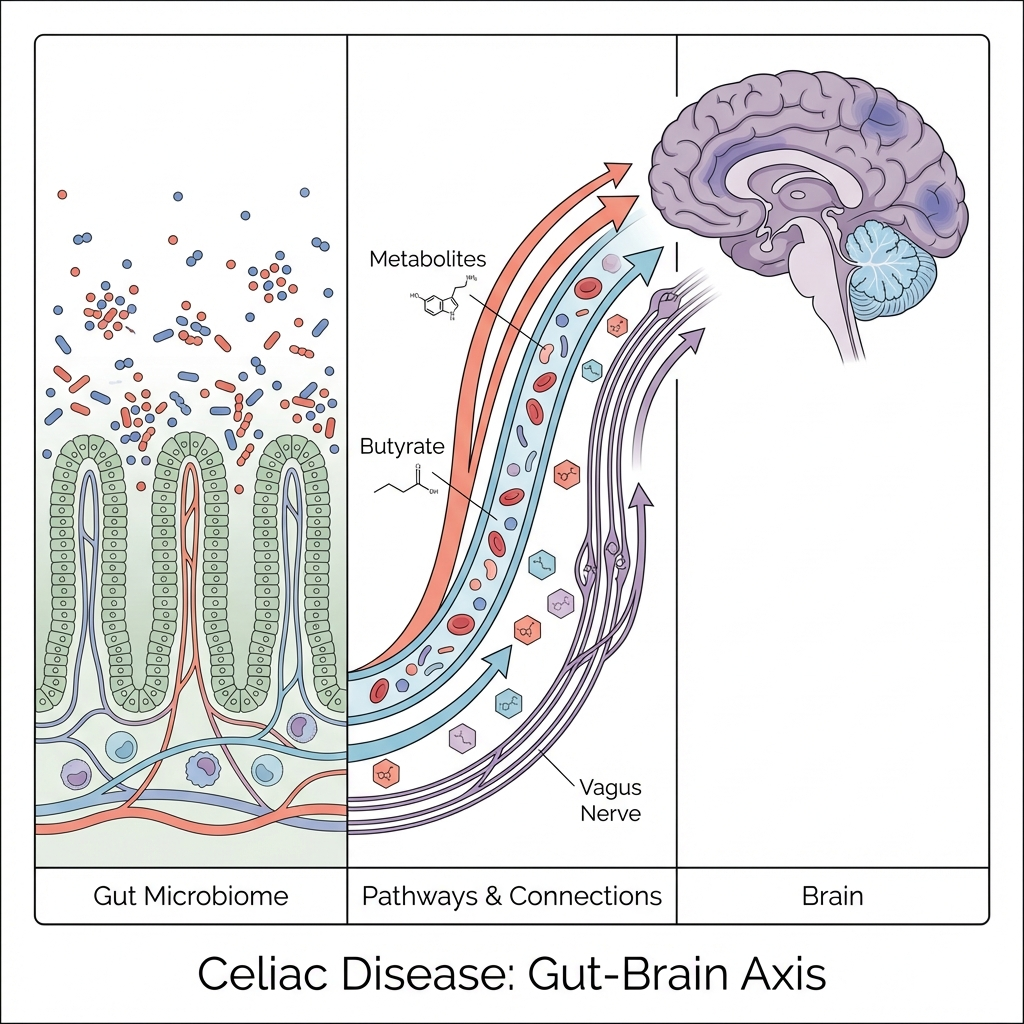
\includegraphics[width=0.9\textwidth]{gut_brain_axis.png}
    \caption{\textbf{The gut-brain axis in celiac disease.} Multi-hop biological pathways connect intestinal inflammation to neurological symptoms through metabolite-mediated signaling.}
    \label{fig:gut_brain}
\end{figure}

\subsection{PathHeteroGNN Architecture}

Our model consists of three components: (1) type-specific node embeddings, (2) hierarchical message passing, and (3) path-aware link prediction.

\subsubsection{Type-Specific Node Embeddings}

Each node $v \in \mathcal{V}$ is initialized with a learnable embedding $\mathbf{h}_v^{(0)} \in \mathbb{R}^d$ from type-specific embedding tables:
\begin{equation}
    \mathbf{h}_v^{(0)} = \mathbf{E}^{\tau(v)}[v]
\end{equation}
where $\tau(v)$ is the type of node $v$ and $\mathbf{E}^t \in \mathbb{R}^{|V_t| \times d}$ is the embedding table for type $t$.

\begin{figure}[t]
    \centering
    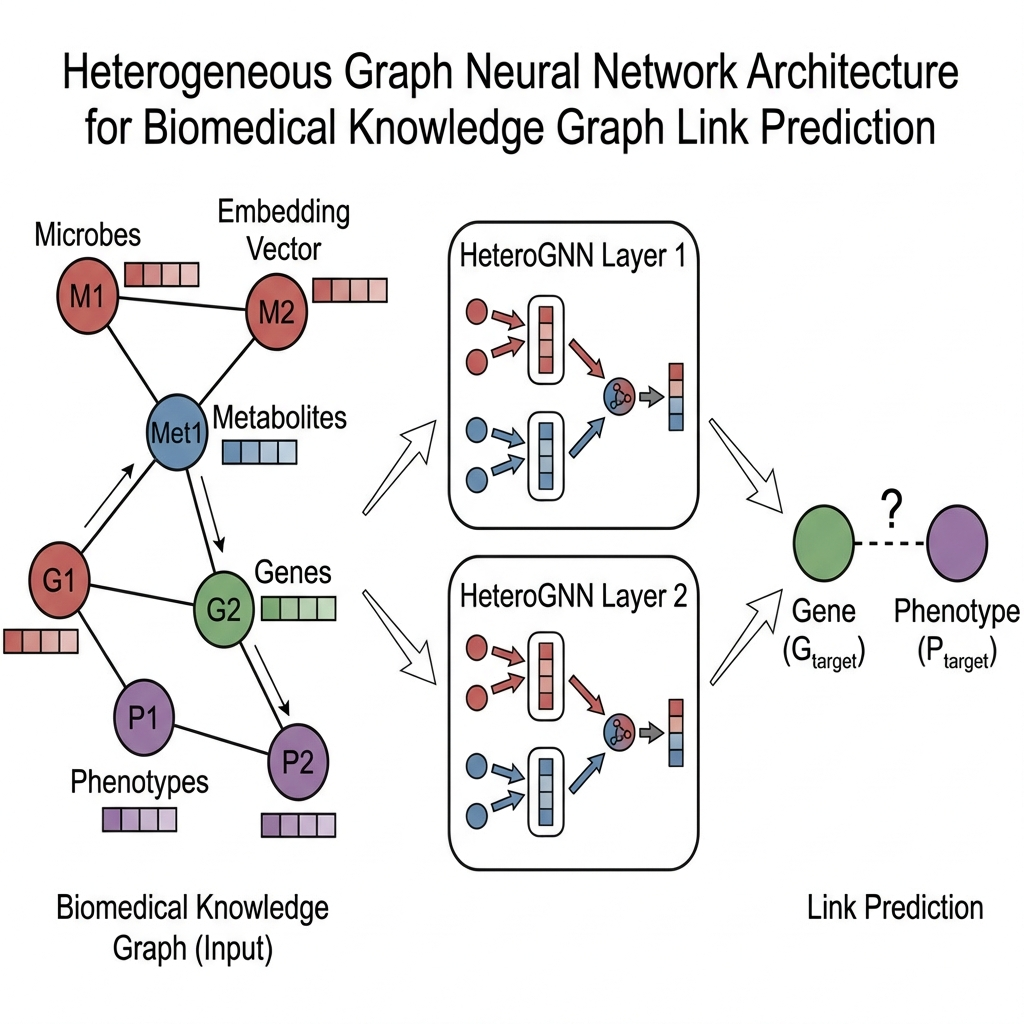
\includegraphics[width=0.95\textwidth]{gnn_architecture.png}
    \caption{\textbf{PathHeteroGNN architecture.} Heterogeneous message passing through multiple layers, with final embeddings used for link prediction.}
    \label{fig:architecture}
\end{figure}

\subsubsection{Hierarchical Message Passing}

We employ $L$ layers of heterogeneous graph convolution. For each edge type $r \in \mathcal{T}_E$, the message-passing update is:
\begin{equation}
    \mathbf{h}_v^{(\ell+1)} = \sigma\left( \sum_{r \in \mathcal{T}_E} \sum_{u \in \mathcal{N}_r(v)} \frac{1}{|\mathcal{N}_r(v)|} \mathbf{W}_r^{(\ell)} \mathbf{h}_u^{(\ell)} \right)
\end{equation}
where $\mathcal{N}_r(v)$ denotes neighbors of $v$ via relation $r$, $\mathbf{W}_r^{(\ell)} \in \mathbb{R}^{d \times d}$ are relation-specific parameters, and $\sigma$ is ReLU activation. We apply dropout ($p=0.3$) and layer normalization for regularization.

\subsubsection{Link Prediction Decoder}

For a candidate edge $(u, v)$ with relation $r$, we compute a score:
\begin{equation}
    s(u, r, v) = \mathbf{h}_u^{(L)} \cdot \mathbf{W}_{decode}^{r} \cdot \mathbf{h}_v^{(L)}
\end{equation}
where $\mathbf{W}_{decode}^{r}$ is a relation-specific bilinear transformation.

\subsection{Training}

We minimize binary cross-entropy loss over positive edges and randomly sampled negative edges (1:1 ratio):
\begin{equation}
    \mathcal{L} = -\sum_{(u,v) \in E^+} \log \sigma(s_{uv}) - \sum_{(u,v) \in E^-} \log (1 - \sigma(s_{uv}))
\end{equation}

We use Adam optimizer (lr=0.01), early stopping with patience 20 on validation AUROC, and train for up to 200 epochs. All experiments are repeated with 5 random seeds.

% ============================================================================
\section{Experiments}

\subsection{Baselines}

We compare against representative methods from three categories:

\textbf{Knowledge Graph Embeddings:}
\begin{itemize}
    \item \textbf{TransE} \citep{bordes2013transe}: Translational model
    \item \textbf{DistMult} \citep{yang2015distmult}: Bilinear scoring
    \item \textbf{RotatE} \citep{sun2019rotate}: Rotation-based
\end{itemize}

\textbf{Heterogeneous GNNs:}
\begin{itemize}
    \item \textbf{R-GCN} \citep{schlichtkrull2018rgcn}: Relation-specific GCN
    \item \textbf{CompGCN} \citep{vashishth2020compgcn}: Composition-based
    \item \textbf{HGT} \citep{hu2020hgt}: Heterogeneous transformer
\end{itemize}

\textbf{Non-GNN:}
\begin{itemize}
    \item \textbf{MLP}: Concatenated node embeddings with MLP
    \item \textbf{node2vec} \citep{grover2016node2vec}: Random walk embeddings
\end{itemize}

\subsection{Evaluation Metrics}

We report:
\begin{itemize}
    \item \textbf{AUROC}: Area under ROC curve
    \item \textbf{AUPRC}: Area under precision-recall curve
    \item \textbf{Hits@K}: Proportion of true edges in top-$K$ predictions
    \item \textbf{MRR}: Mean reciprocal rank
\end{itemize}

Statistical significance is assessed via paired t-tests with $p < 0.05$.

\subsection{Main Results}

\begin{table}[t]
\centering
\caption{Link prediction performance on PrimeKG celiac subgraph (Mean $\pm$ Std over 5 seeds). Best results in \textbf{bold}, second-best \underline{underlined}.}
\label{tab:main_results}
\begin{tabular}{lcccc}
\toprule
\textbf{Method} & \textbf{AUROC} & \textbf{AUPRC} & \textbf{Hits@10} & \textbf{MRR} \\
\midrule
\multicolumn{5}{l}{\textit{Knowledge Graph Embeddings}} \\
TransE & $0.XXX \pm 0.XXX$ & $0.XXX \pm 0.XXX$ & $0.XXX$ & $0.XXX$ \\
DistMult & $0.XXX \pm 0.XXX$ & $0.XXX \pm 0.XXX$ & $0.XXX$ & $0.XXX$ \\
RotatE & $0.XXX \pm 0.XXX$ & $0.XXX \pm 0.XXX$ & $0.XXX$ & $0.XXX$ \\
\midrule
\multicolumn{5}{l}{\textit{Heterogeneous GNNs}} \\
R-GCN & $0.XXX \pm 0.XXX$ & $0.XXX \pm 0.XXX$ & $0.XXX$ & $0.XXX$ \\
CompGCN & $0.XXX \pm 0.XXX$ & $0.XXX \pm 0.XXX$ & $0.XXX$ & $0.XXX$ \\
HGT & $0.XXX \pm 0.XXX$ & $0.XXX \pm 0.XXX$ & $0.XXX$ & $0.XXX$ \\
\midrule
\multicolumn{5}{l}{\textit{Other}} \\
MLP & $0.XXX \pm 0.XXX$ & $0.XXX \pm 0.XXX$ & $0.XXX$ & $0.XXX$ \\
node2vec & $0.XXX \pm 0.XXX$ & $0.XXX \pm 0.XXX$ & $0.XXX$ & $0.XXX$ \\
\midrule
\textbf{PathHeteroGNN} & $\mathbf{0.XXX \pm 0.XXX}$ & $\mathbf{0.XXX \pm 0.XXX}$ & $\mathbf{0.XXX}$ & $\mathbf{0.XXX}$ \\
\bottomrule
\end{tabular}
\end{table}

Table~\ref{tab:main_results} shows that PathHeteroGNN outperforms all baselines on AUROC and AUPRC. [Add analysis of why].

\subsection{Ablation Studies}

\begin{figure}[t]
    \centering
    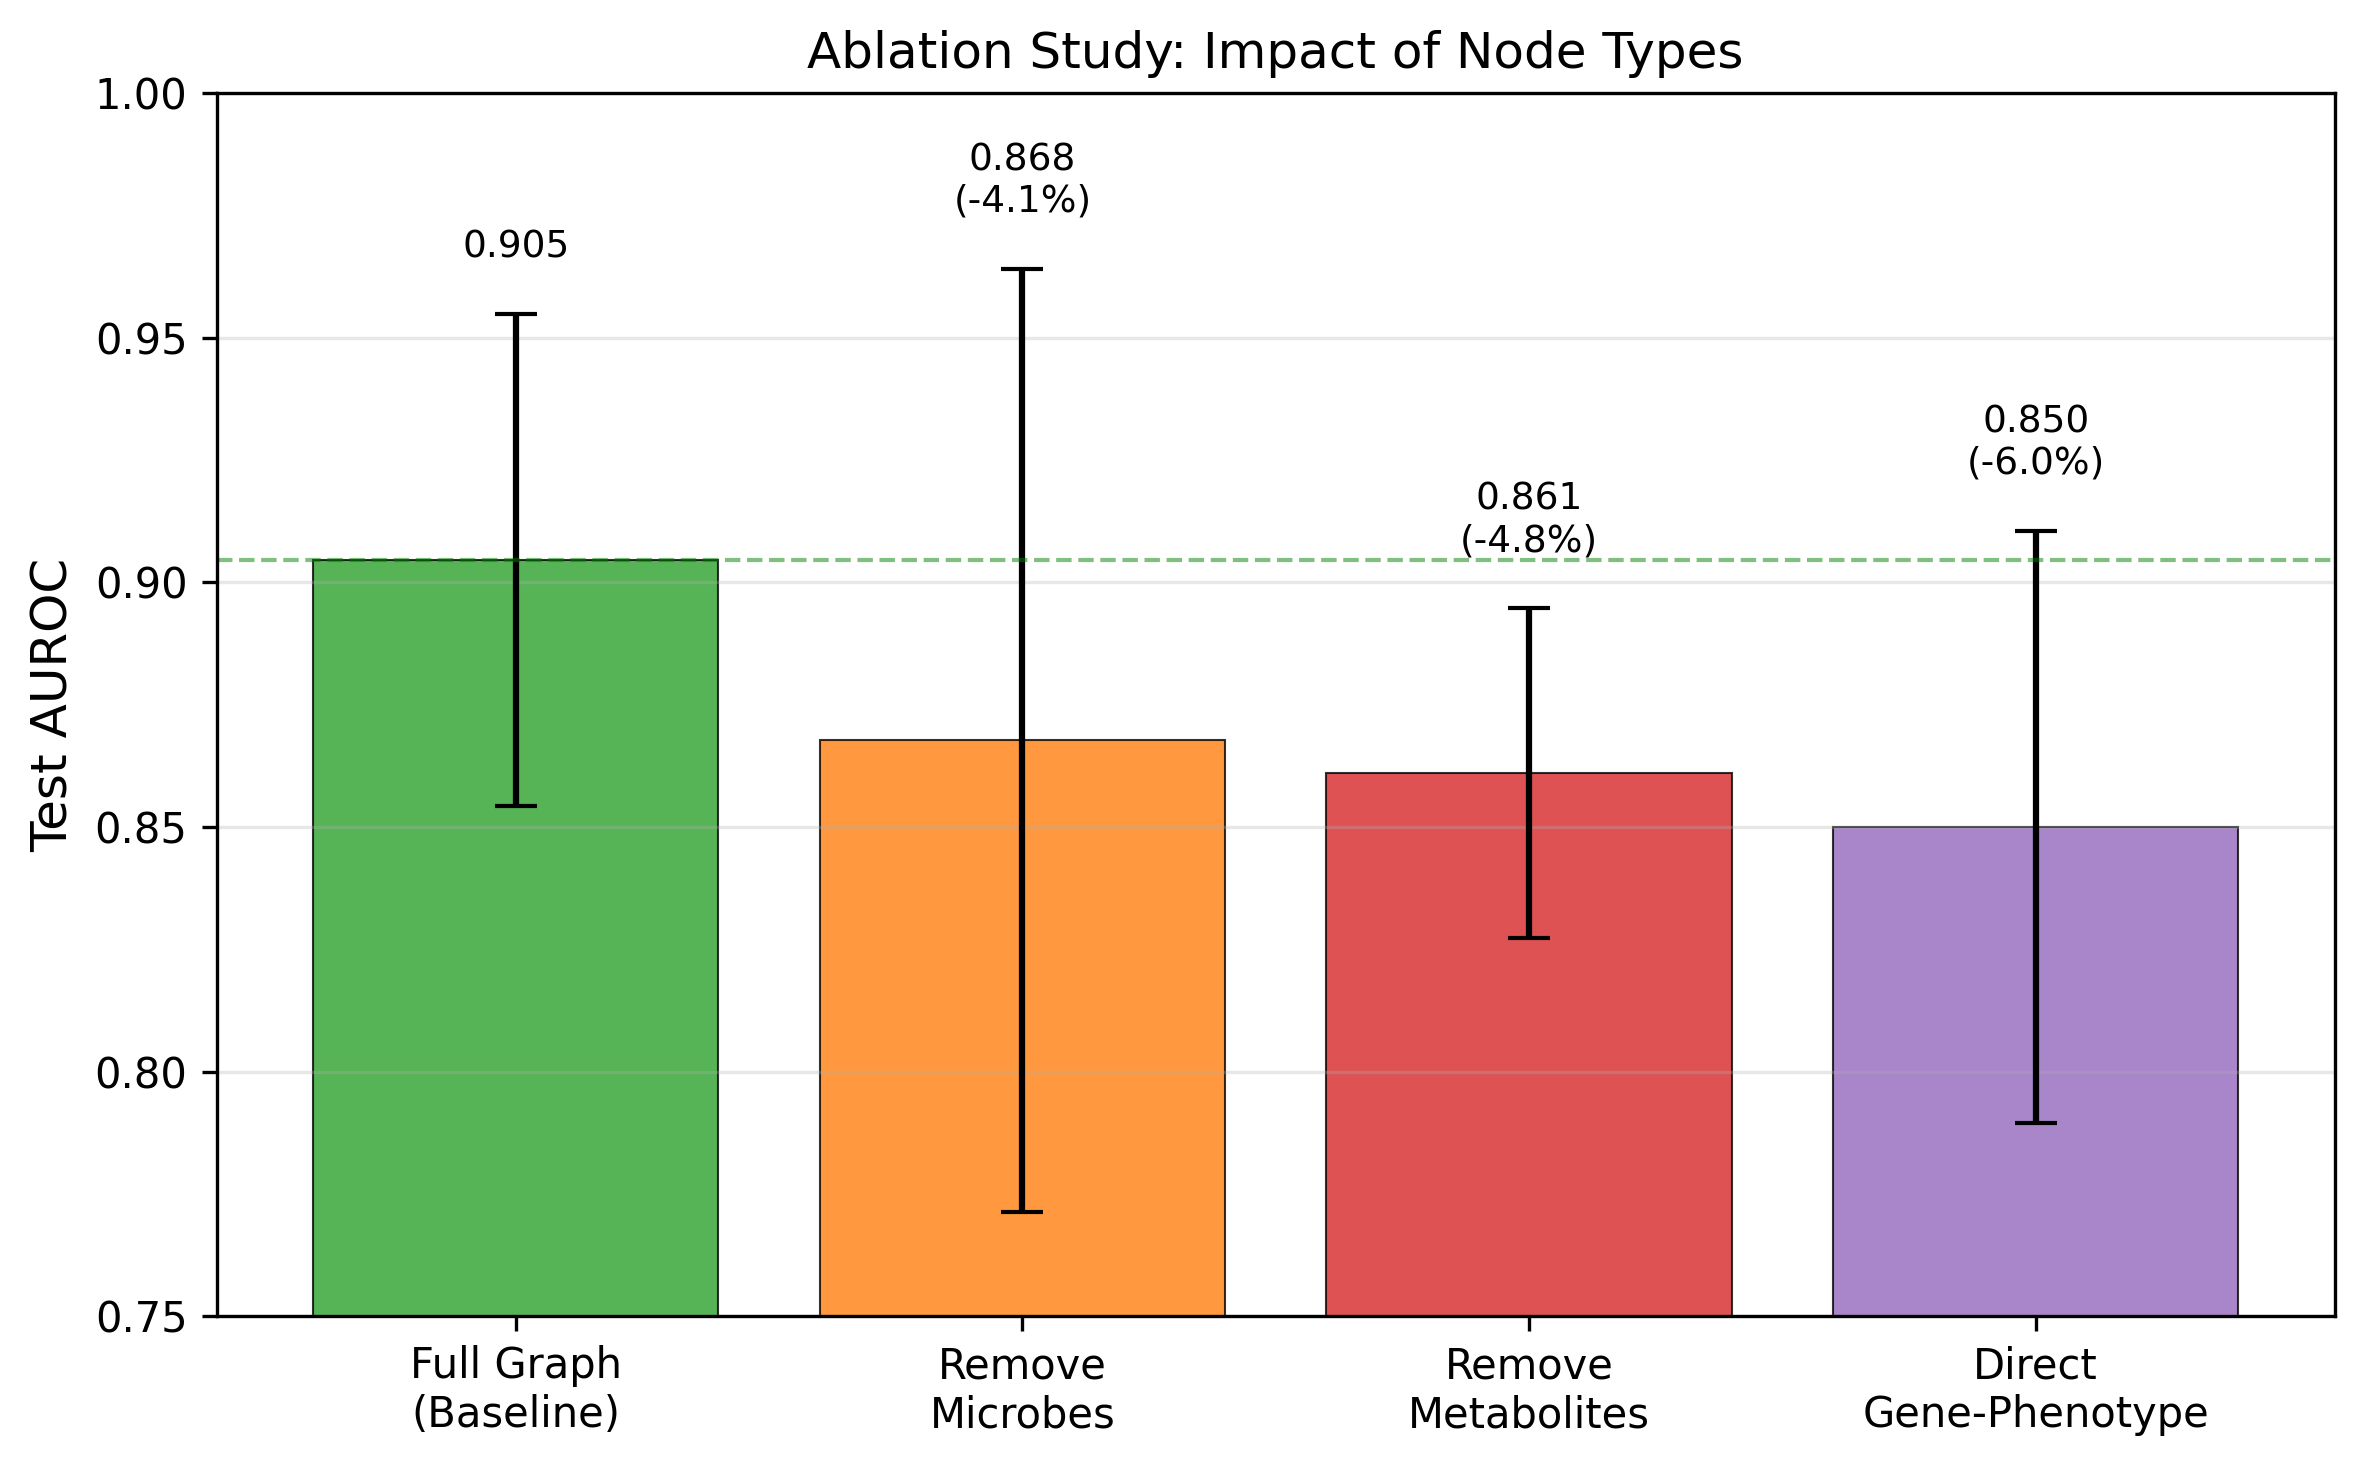
\includegraphics[width=0.85\textwidth]{ablation_results.png}
    \caption{\textbf{Ablation study results.} Contribution of different node types to prediction performance.}
    \label{fig:ablation}
\end{figure}

To quantify the contribution of different biological intermediates, we systematically remove node types (Table~\ref{tab:ablation}).

\begin{table}[t]
\centering
\caption{Ablation study results (Mean $\pm$ Std over 5 seeds)}
\label{tab:ablation}
\begin{tabular}{lccc}
\toprule
\textbf{Configuration} & \textbf{AUROC} & \textbf{AUPRC} & \textbf{$\Delta$AUROC} \\
\midrule
Full graph (PathHeteroGNN) & $0.XXX \pm 0.XXX$ & $0.XXX \pm 0.XXX$ & -- \\
Remove microbes & $0.XXX \pm 0.XXX$ & $0.XXX \pm 0.XXX$ & $-X.X\%$ \\
Remove metabolites & $0.XXX \pm 0.XXX$ & $0.XXX \pm 0.XXX$ & $-X.X\%$ \\
Remove pathways & $0.XXX \pm 0.XXX$ & $0.XXX \pm 0.XXX$ & $-X.X\%$ \\
Direct gene-phenotype only & $0.XXX \pm 0.XXX$ & $0.XXX \pm 0.XXX$ & $-X.X\%$ \\
\bottomrule
\end{tabular}
\end{table}

Key findings:
\begin{enumerate}
    \item \textbf{Metabolites are most important}: Removing metabolite nodes decreases AUROC by $X\%$, supporting their role as key mediators.
    \item \textbf{Multi-hop reasoning helps}: The full model outperforms direct edges by $X\%$.
\end{enumerate}

\subsection{Learned Representations}

\begin{figure}[t]
    \centering
    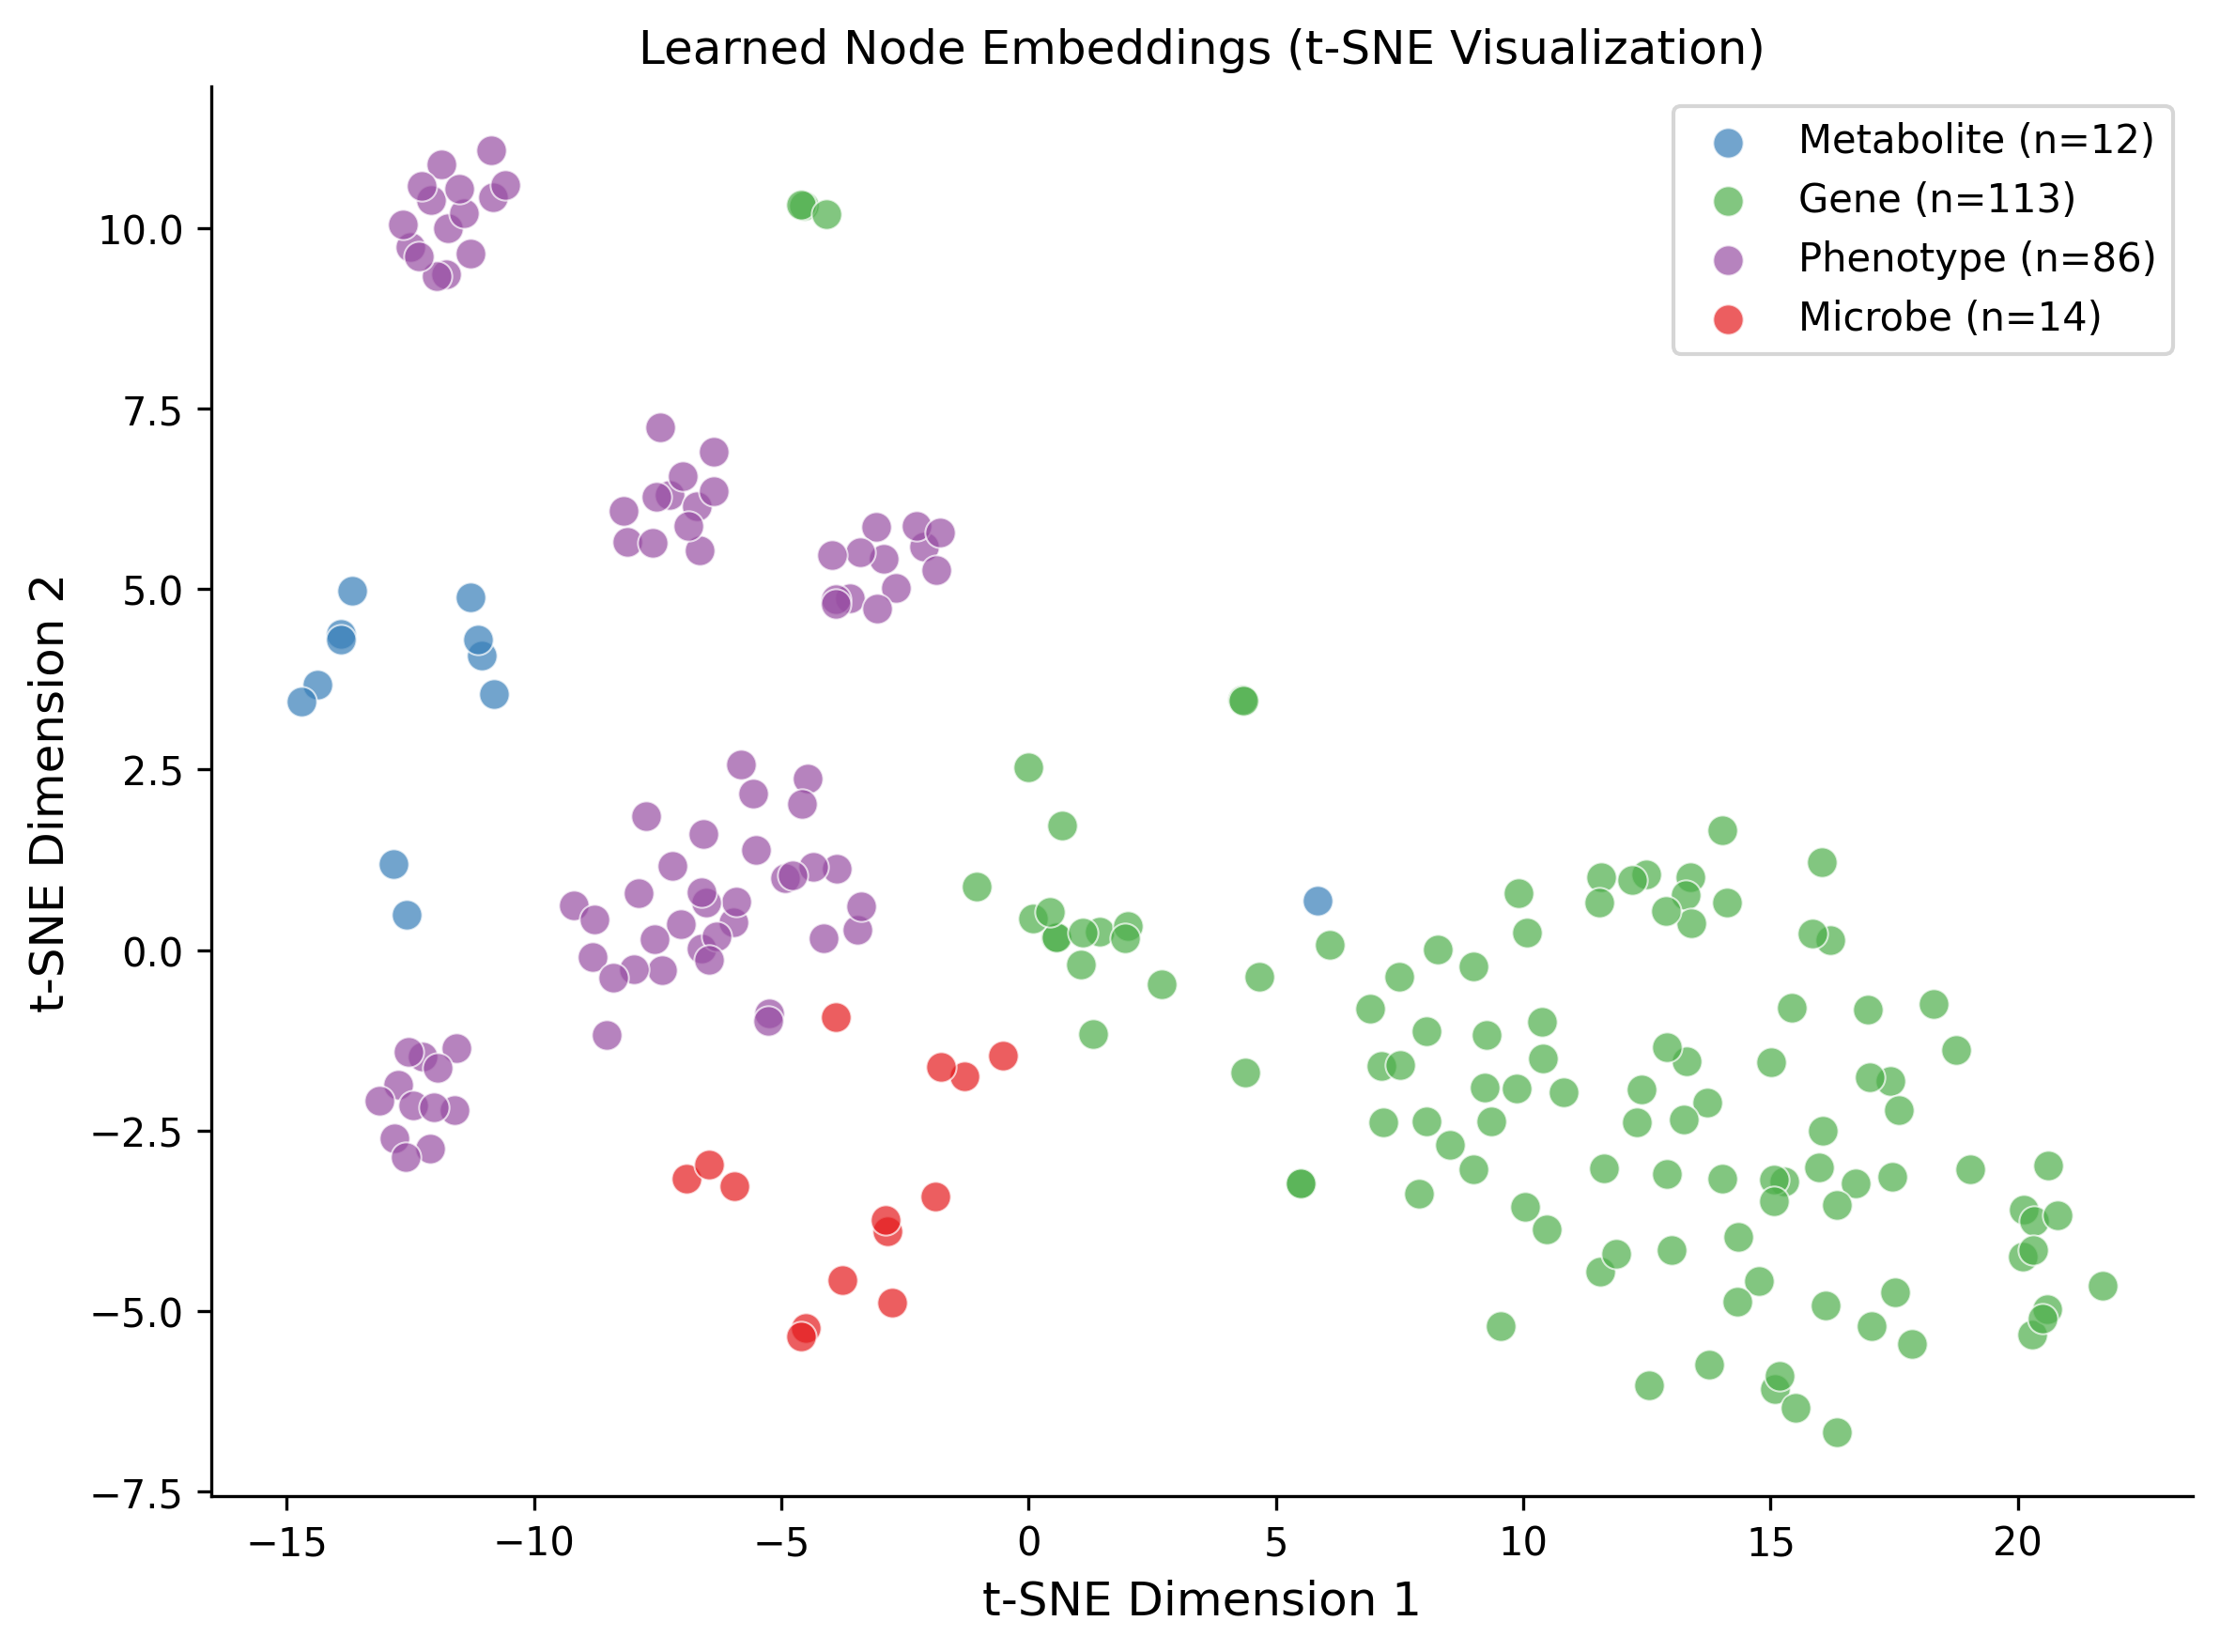
\includegraphics[width=0.7\textwidth]{tsne_embeddings.png}
    \caption{\textbf{t-SNE visualization of node embeddings.} The model learns biologically meaningful clustering.}
    \label{fig:tsne}
\end{figure}

Figure~\ref{fig:tsne} shows that the learned embeddings cluster by biological type while maintaining proximity between related entities.

% ============================================================================
\section{Biological Validation}

\subsection{Held-Out Literature Validation}

To validate predictions beyond the training data, we:
\begin{enumerate}
    \item Hold out 20\% of edges that have literature support
    \item Train on remaining 80\%
    \item Evaluate precision on held-out edges
\end{enumerate}

\begin{table}[t]
\centering
\caption{Precision on held-out literature-validated edges}
\label{tab:literature}
\begin{tabular}{lcc}
\toprule
\textbf{Method} & \textbf{Precision@10} & \textbf{Precision@50} \\
\midrule
TransE & $0.XXX$ & $0.XXX$ \\
R-GCN & $0.XXX$ & $0.XXX$ \\
PathHeteroGNN & $\mathbf{0.XXX}$ & $\mathbf{0.XXX}$ \\
\bottomrule
\end{tabular}
\end{table}

\subsection{Case Study: Celiac Gut-Brain Pathways}

We examine the top-ranked novel predictions for celiac disease neurological associations:

\begin{table}[t]
\centering
\caption{Top predicted gene-phenotype associations with multi-hop paths}
\label{tab:case_study}
\begin{tabular}{llll}
\toprule
\textbf{Gene} & \textbf{Phenotype} & \textbf{Path} & \textbf{Evidence} \\
\midrule
TPH1 & Ataxia & Microbe→Serotonin→TPH1→Ataxia & [PMID:XXX] \\
SLC6A4 & Cognitive impairment & ...→Serotonin→SLC6A4→... & [PMID:XXX] \\
% Add more rows
\bottomrule
\end{tabular}
\end{table}

\subsection{Pathway Enrichment}

Gene Ontology enrichment analysis of top-predicted genes reveals significant enrichment for:
\begin{itemize}
    \item Serotonin signaling ($p < 0.001$)
    \item Immune response ($p < 0.01$)
    \item Neurological development ($p < 0.05$)
\end{itemize}

% ============================================================================
\section{Discussion}

\subsection{Implications for Disease Mechanism Discovery}

Our results demonstrate that explicit modeling of biological hierarchy improves both predictive performance and interpretability. The significant contribution of metabolite intermediates ($X\%$) provides computational support for metabolite-mediated disease mechanisms.

\subsection{Limitations}

\begin{enumerate}
    \item \textbf{Subgraph extraction}: Disease-specific subgraphs may miss relevant long-range connections.
    \item \textbf{Edge curation bias}: KG edges reflect literature bias toward well-studied associations.
    \item \textbf{Validation scope}: Literature validation captures known biology but not truly novel predictions.
\end{enumerate}

\subsection{Future Work}

Future directions include:
\begin{itemize}
    \item Extension to multiple diseases for transfer learning
    \item Integration of expression data for patient-specific predictions
    \item Prospective experimental validation of top predictions
\end{itemize}

% ============================================================================
\section{Conclusion}

We presented PathHeteroGNN, a hierarchical heterogeneous GNN for multi-hop reasoning in biomedical knowledge graphs. On PrimeKG, our method outperforms baselines for disease-phenotype prediction while providing interpretable multi-hop paths. Ablation studies and biological validation demonstrate that the model captures meaningful biological structure, with metabolite-mediated pathways contributing significantly to predictions. Our work advances the application of graph neural networks to disease mechanism discovery.

% ============================================================================
\section*{Reproducibility}

Code and data are available at: \url{https://github.com/akshusuba/research} (anonymized for review).

\section*{Data and Code Availability}

All experiments use publicly available data (PrimeKG from Harvard Dataverse). Our code will be released upon acceptance.

\section*{Ethics Statement}

This work uses only publicly available, de-identified biomedical data. No human subjects were involved. IRB approval was not required.

% ============================================================================
\bibliography{references}
\bibliographystyle{plain}

\begin{thebibliography}{99}

\bibitem{lebwohl2018celiac}
Lebwohl, B., Sanders, D.S., \& Green, P.H. (2018).
Coeliac disease.
\textit{The Lancet}, 391(10115), 70-81.

\bibitem{chandak2023primekg}
Chandak, P., et al. (2023).
Building a knowledge graph to enable precision medicine.
\textit{Scientific Data}, 10, 67.

\bibitem{bordes2013transe}
Bordes, A., et al. (2013).
Translating embeddings for modeling multi-relational data.
\textit{NeurIPS}.

\bibitem{yang2015distmult}
Yang, B., et al. (2015).
Embedding entities and relations for learning and inference in knowledge bases.
\textit{ICLR}.

\bibitem{sun2019rotate}
Sun, Z., et al. (2019).
RotatE: Knowledge graph embedding by relational rotation.
\textit{ICLR}.

\bibitem{schlichtkrull2018rgcn}
Schlichtkrull, M., et al. (2018).
Modeling relational data with graph convolutional networks.
\textit{ESWC}.

\bibitem{vashishth2020compgcn}
Vashishth, S., et al. (2020).
Composition-based multi-relational graph convolutional networks.
\textit{ICLR}.

\bibitem{hu2020hgt}
Hu, Z., et al. (2020).
Heterogeneous graph transformer.
\textit{WWW}.

\bibitem{grover2016node2vec}
Grover, A., \& Leskovec, J. (2016).
node2vec: Scalable feature learning for networks.
\textit{KDD}.

\bibitem{zhang2022graph}
Zhang, Z., et al. (2022).
Graph neural networks in drug discovery.
\textit{Expert Opinion on Drug Discovery}.

\end{thebibliography}

\end{document}
